%----------------------------------------------------------------------------------------
%	SECTION 1.1
%----------------------------------------------------------------------------------------

\section{Compact Subspaces of $\R$.}

We now construct new compact spaces from old ones and prove some results from
real analysis.

\begin{theorem}\label{3.6.1}
    Let $X$ be a simply ordered set satisfying the least upper bound property.
    Then every closed interval in $X$ is compact under the order topology.
\end{theorem}
\begin{proof}
    Let $a<b$ for  $a,b \in X$ and let  $\Ac$ be an open covering of  $[a,b]$ of
    sets open in $[a,b]$ under the subspace topology. Let $x \in [a,b]$ with $x
    \neq b$, and suppose that $x$ has an immediate successor  $y>x$, that is
    there is no $z \in [a,b]$ with $y>z>x$. Then $[x,y]=\{x,y\}$ so it can be
    covered by at most two elements of  $\Ac$. Now, if no such  $y$ exists in
    $X$, then choose an  $A \in \Ac$ with  $x \in A$, since  $x \neq b$, we get
    that  $A$ is open, and that  $A$ contains an interval of the form  $[x,c)$
    for some $c \in [a,b]$, with $x < c$. Then choose a point  $y \in (x,y)$
    then the interval $[x,y]$ is covered by $A$, since $x<y<c$.

    Now let $C$ be the set of all  $y>a$ of  $[a,b]$ such that the interval
    $[a,y]$ is covered by finitely many elements of $\Ac$. By the above case
    there exists at least one such  $y$, so that  $C \neq \emptyset$. Now, let
    $c$ be the least upperbound of  $C$, then  $a<c \leq b$.

    Now, choose an element $A \in \Ac$ with $c \in A$. Since $A$ is open, it
    contains an interval of the form  $(d,c]$ for some $d \in [a,b]$. Now, if $c
    \notin C$ then there exists a  $z \in C$ with  $z \in (d,c)$; for otherwise,
    $d$ would be an upperbound of $C$ which cannot happen. Then $[z,c]$ can be
    covered by $n$ elements of $\Ac$. Now,  $[z.c] \subseteq A$, so
    $[a,c]=[a,z] \cup [z,c]$ can be covered by $n+1$ elements of  $\Ac$, which
    puts  $c \in C$; which contradicts that  $c \notin C$.

    Now suppose that  $c<b$ then by the first argument, with  $x=c$ there is a
    $y>c$ of  $[a,b]$ such that $[c,y]$ can be covered by finitely many elements
    of $\Ac$. Since  $c \in C$, we have that $[a,c]$ can also be covered by
    finitely many elements of $\Ac$; so then can the interval
    \begin{equation*}
        [a,y] = [a,c] \cup [c,y]
    \end{equation*}
    This makes $y \in C$, which cotradicts that  $c$ is the least upperbound of
     $C$. Therefore, $X$ must be compact.
\end{proof}
\begin{corollary}
    Every closed interval in $\R$ is compact.
\end{corollary}

\begin{theorem}\label{3.6.2}
    A subspace $A$ of  $\R^n$ is compact if, and only if it is closed and  is
    bounded in the Euclidean metric or the Square metric.
\end{theorem}
\begin{proof}
    Let $\rho$ the Square metric. Then recall that:
    \begin{equation}
        \rho(x,y) \leq \|x-y\| \leq \rho(x,y)\sqrt{n}
    \end{equation}
    This inequality implies that the subspace $A$ is bounded under  $\|\cdot\|$
    if and only if it is bounded under  $\rho$.

    Now suppose that  $A$ is compact. Since  $\R^n$ is Hausdorff, by theorem
    \ref{3.4.3}, $A$ is closed. Consider the the collection of all open balls
    $B_\rho(0,m)$ where $m \in \Z^+$ whose union of elements is all of $\R^n$,
    that is:
    \begin{equation*}
        \R^n = \bigcup_{m \in \Z^+}{B_\rho(0,m)}
    \end{equation*}
    By hypothesis, some finite subcollection covers $A$. Then we have that for
    some  $M$, $A \subseteq B_\rho(0,M)$; then for any two points $x,y \in A$,
    $\rho(x,y) \leq 2M$, which bounds $A$ under  $\rho$. Now,since $\rho(x,y)
    \leq \|x-y\|$, this makes $A$ bounded under $\|\cdot\|$.

    Conversely, supposed that  $A$ is closed, and bounded under  $\rho$ (and
    consequently $\|\cdot\|$), and that $\rho(x,y) \leq N$ for all $x,y \in A$.
    Now, choose an  $x_0 \in A$ such that $\rho(x_0,0)=b$, then by the triangle
    inequality, $\rho(x,0) \leq \rho(x,x_0)+\rho(x_0,0)=N+b$ for all $x \in A$.
    Now, we get that $A$ is a subset of the cube $[-b-N,N+b]$ which is compact
    in $\R$. Since  $A$ is closed, we get that  $A$ is compact.
\end{proof}

\begin{example}\label{3.10}
    \begin{enumerate}
        \item[(1)] The unit ball $S^{n-1}$ and closed unit ball $B^n$ in  $\R^n$
            are compact by the above theorem, since they are both closed and
            bouned.

        \item[(2)] The curve $A=\{x \times \frac{1}{x} : 0 < x \leq 1\}$ in
            $\R^2$ is closed, but not bounded, so it is not compact by the above
            theorem.

        \item[(3)] The curve $A=\{x \times \sin{\frac{1}{x}} : 0 < x \leq 1\}$
            in $\R^2$ is bounded, but not closed, so it is not compact.
    \end{enumerate}
\end{example}

\begin{theorem}[The Extreme Value Theorem]\label{3.6.3}
    $X$ be a topological space, and  Let $Y$ be an ordered set under the order
    topology, and let $f:X \rightarrow Y$ be a continuous finction. If $X$ is
    compact, then there exist points  $c,d \in X$ such that  $f(c) \leq f(x)
    \leq f(d)$ for all $x \in X$.
\end{theorem}
\begin{proof}
    Suppose that $X$ is compact, then since  $f$ is continuous, then $A=f(X)$ is
    compact by theorem \ref{3.4.4}. Now if  $A$ has no largest element,
    then the collection of all rays $\Ac=\{(-\infty,a) : a \in A\}$ forms an
    open covering of $A$, then by compactness, there is a finite subcollection
    $\{(-\infty,a_1), \dots, (-\infty,a_n)\}$ that covers $A$. If  $a_i$ is the
    largest element, then  $a_i$ is in none of these sets, which contradicts
    that they cover  $A$. Then $A$ has a largest element  $M=f(d)$ for some $d
    \in X$.

    By similar reasoning, taking  $\Ac=\{(a,\infty) : a \in A\}$, we see that
    $A$ has a smallest element  $m=f(c)$ for $c \in X$.
\end{proof}

\begin{definition}
    Let $X$ be a metric space with metric $d$, and let  $A \subseteq X$ be
    nonempty. For each  $x \in X$, we define the  \textbf{distance} from $x$ to
     $A$ to be:
     \begin{equation}
         d(x,A) = \inf\{d(x,a) : a \in A\}
     \end{equation}
     That is, it is the greatest lowerbound of all the distances between $x$ and
     elements of $A$.
\end{definition}

\begin{lemma}\label{3.6.4}
    Let $X$ be a metric space with metric $d$, and $A \subseteq X$ nonempty,
    then for all  $x \in X$,  $d(x,A)$ is a continuous function.
\end{lemma}
\begin{proof}
    Fix $x \in X$ and take  $y \in X$. Then by definition and the triangle
    inequality:
    \begin{equation*}
        d(x,A) \leq d(x,a) \leq d(x,y)+d(y,a)
    \end{equation*}
    for each $a \in A$, so we get:
    \begin{equation*}
        d(x,A)-d(x,y) \leq \inf{d(y,a)}=d(y,A)
    \end{equation*}
    and so $d(x,A)$ is continuous.
\end{proof}
\begin{remark}
    Do not understand, please work thriugh the proof and rewrite it.
\end{remark}

\begin{lemma}[The Lebesgue Number Lemma]\label{3.6.5}
    Let $\Ac$ be an open covering of a metric space $X$ with metric $d$. If $X$
    is compact, then there exists a  $\delta>0$ such that for each subset of
    $X$ with diameter less than  $\delta$, there exists an element of  $\Ac$
    containing it.
\end{lemma}
\begin{proof}
    Let $\Ac$ be an open covering of  $X$. If  $X \in \Ac$, then any positive
    real number is a Lebesgue number for  $\Ac$. Now, suppose that  $X \notin
    \Ac$. Then choose a finite subcollection  $\{A_1, \dots, A_n\}$ of $\Ac$
    covering  $X$. Then for each  $i$, let  $C_i=\com{X}{A_i}$ and define $f:X
    \rightarrow \R$ by the rule:
    \begin{equation}
        f(x) = \frac{1}{n}\sum_{i=1}^{n}{d(x,C_i)}
    \end{equation}
    Then $f(x)>0$ for all $x \in X$; for, fix $x$ and choose an  $i$ so that
    $x \in A_i$, and choose $\epsilon$ so that $B_d(x,\epsilon) \subseteq A_i$,
    then  $d(x,C_i) \geq \epsilon$ so that $f(x)>\frac{\epsilon}{n}$.

    Now, we have $f$ is continuous since  $d(x,C_i)$ is continuous. Then $f$ has
    minimum value  $\delta>0$. Let $B \subseteq A$ have diameter
    $\diam{B}<\delta$ and choose a point $x_0 \in B$. Then $B \subseteq
    B_d(x_0,\delta)$. Now, we have that
    \begin{equation*}
        \delta \leq f(x_0) \leq d(x_0,C_m)
    \end{equation*}
    where $d(x_0,C_m)$ is the largest of the $d(x_0,C_i)$. Then we see that
    $B_d(x_0,\delta) \subseteq A_m=\com{X}{C_m}$.
\end{proof}

\begin{definition}
    Let $\Ac$ be an open covering of a compact metric space $X$ with metric $d$.
    We call a number $\delta>0$ such that for each subseet of  $X$ with
    $\diam<\delta$, there exists an element of  $\Ac$ containing it a
    \textbf{Lebesgue number} of $\Ac$.
\end{definition}

\begin{definition}
    Let $X$ and  $Y$ be metric spaces with metrics $d_X$, and  $d_Y$
    repsectivelty. A function $f:X \rightarrow Y$ is said to be
    \textbf{uniformly continuous} if given $\epsilon>0$, there is a  $\delta>0$
    such that for every pair of points  $x,y \in X$, $d_X(x,y)<\delta$ implies
    that $d_Y(f(x),f(y))<\epsilon$.
\end{definition}

\begin{theorem}[The Uniform Continuity Theorem]\label{3.6.6}
    Let $X$ and  $Y$ be metric spaces with metrics $d_X$, and  $d_Y$
    repsectivelty, and let $X$ be compact. Then the function
    $f:X \rightarrow Y$ is uniformly continuous only if it is continous.
\end{theorem}
\begin{proof}
    Let $\epsilon>0$ and let  $\Ac=\{B(y,\frac{\epsilon}{2})\}_{y \in Y}$ be an
    open covering of $Y$. Then  $f^{-1}(\Ac)=\{f^{-1}(B(y,\frac{\epsilon}{2}))\}$
    is an open covering of $X$. Now, choose $\delta>0$ a Lebesgue number for
    $f^{-1}(\Ac)$, then for $x,z \in X$ with  $d_X(x,x)<\delta$, the set
    $\{x,z\}$ has $\diam\{x,z\}<\delta$, so $\{\f(x),f(z)\} \subseteq
    B(y,\frac{\epsilon}{2})$ for $y \in Y$. Thus  $d_Y(f(x),f(z))<\epsilon$.
\end{proof}

\begin{definition}
    If $X$ is a toplogical space, then a point $x \in X$ is called an
    \textbf{isolated point} if the one-point set $\{x\}$ is open in $X$.
\end{definition}

\begin{figure}[h]
    \centering
    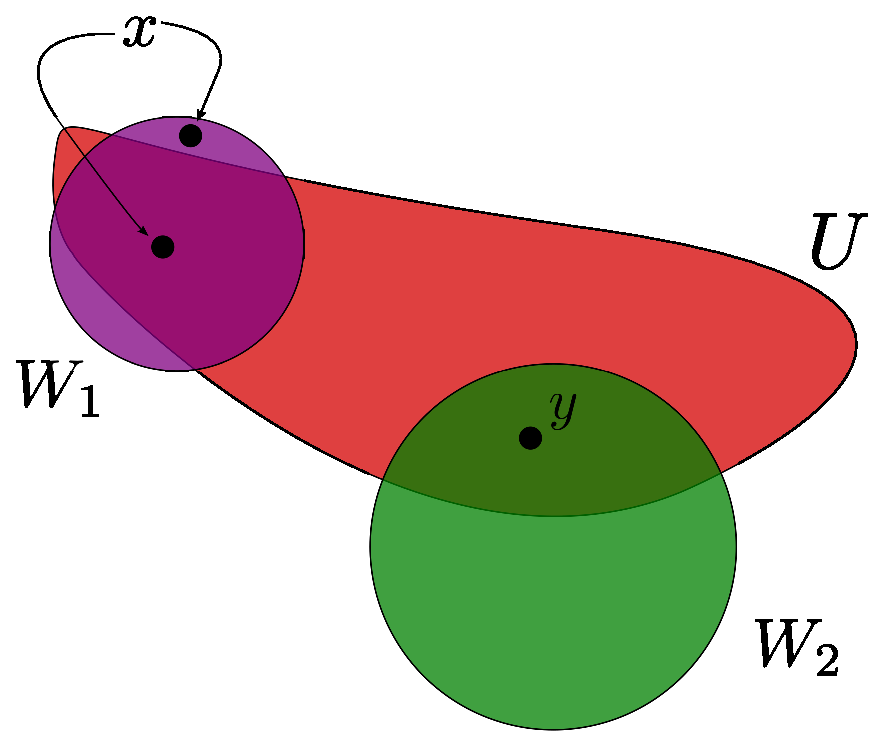
\includegraphics[scale=0.5]{Figures/Chapter3/thm3_6_7.eps}
    \caption{We choose disjoint neighborhoods $W_1$ and  $W_2$ of $x$ and  $y$
    respectively. Here we want  $y \in W_2 \cap U$, but  $x$ may be in  $W_1
\cap U$ or simply $\com{W_1}{U}$.}
    \label{fig_3.4}
\end{figure}

\begin{theorem}\label{3.6.7}
    Let $X$ be a nonepmty compact Hausdorff space. Then if $X$ has no isolated
    points,  $X$ is uncountable.
\end{theorem}
\begin{proof}
    Let $U \neq \emptyset$ be an open set of  $X$, and let  $x \in X$. Choose
    then a  $y \in X$ with  $y \neq x$. Choose also disjoint neighborhoods
    $W_1$, and $W_2$ of $x$ and  $y$, respectively, (figure \ref{fig_3.4}) and
    let  $V=W_2 \cap U$. Then $V \subseteq U$ is nonempty and  $x \notin
    \cl{V}$.

    Now let $f:\Z^+ \rightarrow X$ be a function, and let $x_n=f(n)$. By the
    preceding argument, let $U=X$ and choose  $V_1 \subseteq U$ nonempty such
    that $x_1 \notin \cl{V_1}$ for $x_1 \in X$. Then proceeding inductively,
    we can get find $V_{n+1} \subseteq V_n$ nonempty with $x_n \notin
    \cl{V_{n+1}}$. Now, consider the nested sequence of nonempty sdubsets:
    \begin{equation*}
        \cl{V_1} \supseteq \cl{V_2} \supseteq \dots \supseteq \cl{V_{n+1}}
        \supseteq \dots
    \end{equation*}
    Since $X$ is compact, there is an
    \begin{equation*}
        x \in \bigcap_{i \in \Z^+}{\cl{V_i}}
    \end{equation*}
    Then $x \neq x_n$ since  $x \in \cl{V_n}$ and $x_n \notin \cl{V_n}$. This
    means that $f$ is not onto, and hence $X$ is uncountable.
\end{proof}
\begin{corollary}
    Every closed set in $\R$ is uncountable.
\end{corollary}
